\documentclass{ctexart}
\usepackage{fontspec}
\usepackage{hyperref}

\hypersetup{
    colorlinks=true, % 启用彩色链接
    linkcolor=blue, % 内部链接颜色
    filecolor=blue, % 文件链接颜色
    urlcolor=blue, % 外部 URL 链接颜色
}


% 设置文档字体
\setmainfont{Times New Roman}
\setsansfont{Arial}
\setmonofont{Consolas}

% 设置文档的字体、编码等
\usepackage[UTF8]{ctex}
\usepackage[T1]{fontenc}
\usepackage{listings} % 代码显示
\usepackage{algorithm2e} % 算法排版
\usepackage{xcolor} % 代码高亮
\usepackage{float} % 图表排版
\usepackage{graphicx} % 插入图片

\usepackage{amsmath}
\usepackage{amssymb}
\usepackage{amsfonts}
\usepackage{bm}

% 代码高亮设置
\definecolor{codegreen}{rgb}{0,0.6,0}
\definecolor{codegray}{rgb}{0.5,0.5,0.5}
\definecolor{codepurple}{rgb}{0.58,0,0.82}
\definecolor{backcolour}{rgb}{0.95,0.95,0.92}
\definecolor{codered}{rgb}{0.6,0,0}
\definecolor{codeblue}{rgb}{0,0,0.6}

% Python样式
\lstdefinestyle{mystyle}{
    language=Python,
    backgroundcolor=\color{backcolour},
    commentstyle=\color{codegreen},
    keywordstyle=\color{magenta},
    numberstyle=\tiny\color{codegray},
    stringstyle=\color{codepurple},
    basicstyle=\ttfamily\footnotesize,
    breakatwhitespace=false,
    breaklines=true,
    captionpos=b,
    keepspaces=true,
    numbers=left,
    numbersep=5pt,
    showspaces=false,
    showstringspaces=false,
    showtabs=false,
    tabsize=2
}

% CUDA样式
\lstdefinestyle{cuda}{
    language=C++,
    backgroundcolor=\color{backcolour},
    commentstyle=\color{codegreen},
    keywordstyle=\color{codeblue},
    numberstyle=\tiny\color{codegray},
    stringstyle=\color{codered},
    basicstyle=\ttfamily\footnotesize,
    breaklines=true,
    captionpos=b,
    morekeywords={__global__, __device__, __host__, cudaMalloc, cudaMemcpy, cudaFree},
    keepspaces=true,
    numbers=left,
    numbersep=5pt
}

% Shell样式
\lstdefinestyle{shell}{
    language=bash,
    backgroundcolor=\color{backcolour},
    commentstyle=\color{codegreen},
    keywordstyle=\color{codeblue},
    numberstyle=\tiny\color{codegray},
    stringstyle=\color{codered},
    basicstyle=\ttfamily\footnotesize,
    breaklines=true,
    captionpos=b,
    keepspaces=true,
    numbers=left,
    numbersep=5pt
}

\newenvironment{customquote}{%
  \quote
  \color{gray} % 设置引用文字为灰色
}{%
  \endquote
}

\lstset{style=mystyle}

\title{Mamba的CUDA实现解读}
\author{黄有}
\date{}

\begin{document}

\maketitle

\section{Mamba模型架构}
本文只针对Mamba~\cite{gu2023mamba}核心部分进行解读,Mamba整体架构可以参考:\href{https://zhuanlan.zhihu.com/p/680846351}{一文读懂Mamba},以及Mamba所采用的离散化方式:\href{https://zhuanlan.zhihu.com/p/680534665}{状态空间模型SSM的离散化过程推导}。基于此,本文直接采用最终的离散化形式进行后续的代码解读,具体如下
\begin{equation*}
\begin{split}
    \bm{h}_k &= e^{\Delta A}\bm{h}_{k-1} + \left(e^{\Delta A} - I\right)A^{-1}B\bm{x}_k \\
    \bm{y}_k &= C\bm{h}_k + D\bm{x}_k,
\end{split}
\end{equation*}
其中$\bm{x}_k, \bm{y}_k$可以理解为当前网络层在单个Token(对于NLP任务)上的输入和输出,$k$指定了Token的索引,$\bm{h}_k$是对应于这个Token的隐藏状态(特征),其他变量都是参数(可以固定,也可以随着输入$\bm{x}_k$而变化)。为简化后续内容,设置维度:
\begin{equation*}
\begin{split}
    &\bm{x}_k, \bm{y}_k \in \mathbb{R}^{d}, \\
    &\bm{h}_k \in \mathbb{R}^{n}, \\
    &\Delta \in \mathbb{R}, \\
    &A \in \mathbb{R}^{n\times n}, \\
    &B \in \mathbb{R}^{n\times d}, \\
    &C \in \mathbb{R}^{d\times n}, \\
    &D \in \mathbb{R}^{d\times d}, \\
\end{split}
\end{equation*}
以上是Mamba的理论结构,实际Mamba的实现形式略有变化,以下结合代码进行讲解。

\section{Mamba代码结构}
以下是\href{https://github.com/state-spaces/mamba}{Mamba源码}(更新截止2024年2月24日)的目录结构:
\lstset{style=shell}
\begin{lstlisting}
mamba/
├── csrc
│   └── selective_scan
│       ├── reverse_scan.cuh
│       ├── selective_scan_bwd_bf16_complex.cu
│       ├── selective_scan_bwd_bf16_real.cu
│       ├── selective_scan_bwd_fp16_complex.cu
│       ├── selective_scan_bwd_fp16_real.cu
│       ├── selective_scan_bwd_fp32_complex.cu
│       ├── selective_scan_bwd_fp32_real.cu
│       ├── selective_scan_bwd_kernel.cuh
│       ├── selective_scan_common.h
│       ├── selective_scan.cpp
│       ├── selective_scan_fwd_bf16.cu
│       ├── selective_scan_fwd_fp16.cu
│       ├── selective_scan_fwd_fp32.cu
│       ├── selective_scan_fwd_kernel_comment.cuh
│       ├── selective_scan_fwd_kernel.cuh
│       ├── selective_scan.h
│       ├── static_switch.h
│       └── uninitialized_copy.cuh
├── mamba_ssm
│   ├── __init__.py
│   ├── models
│   │   ├── config_mamba.py
│   │   ├── __init__.py
│   │   └── mixer_seq_simple.py
│   ├── modules
│   │   ├── __init__.py
│   │   └── mamba_simple.py
│   ├── ops
│   │   ├── __init__.py
│   │   ├── selective_scan_interface.py
│   │   └── triton
│   │       ├── __init__.py
│   │       ├── layernorm.py
│   │       └── selective_state_update.py
│   └── utils
│       ├── generation.py
│       ├── hf.py
│       └── __init__.py
├── ...
\end{lstlisting}
以上罗列了源码中和Mamba模型相关部分的目录结构,更具体的代码结构可以参考下面的思维导图:
\begin{figure}[H]
    \centering
    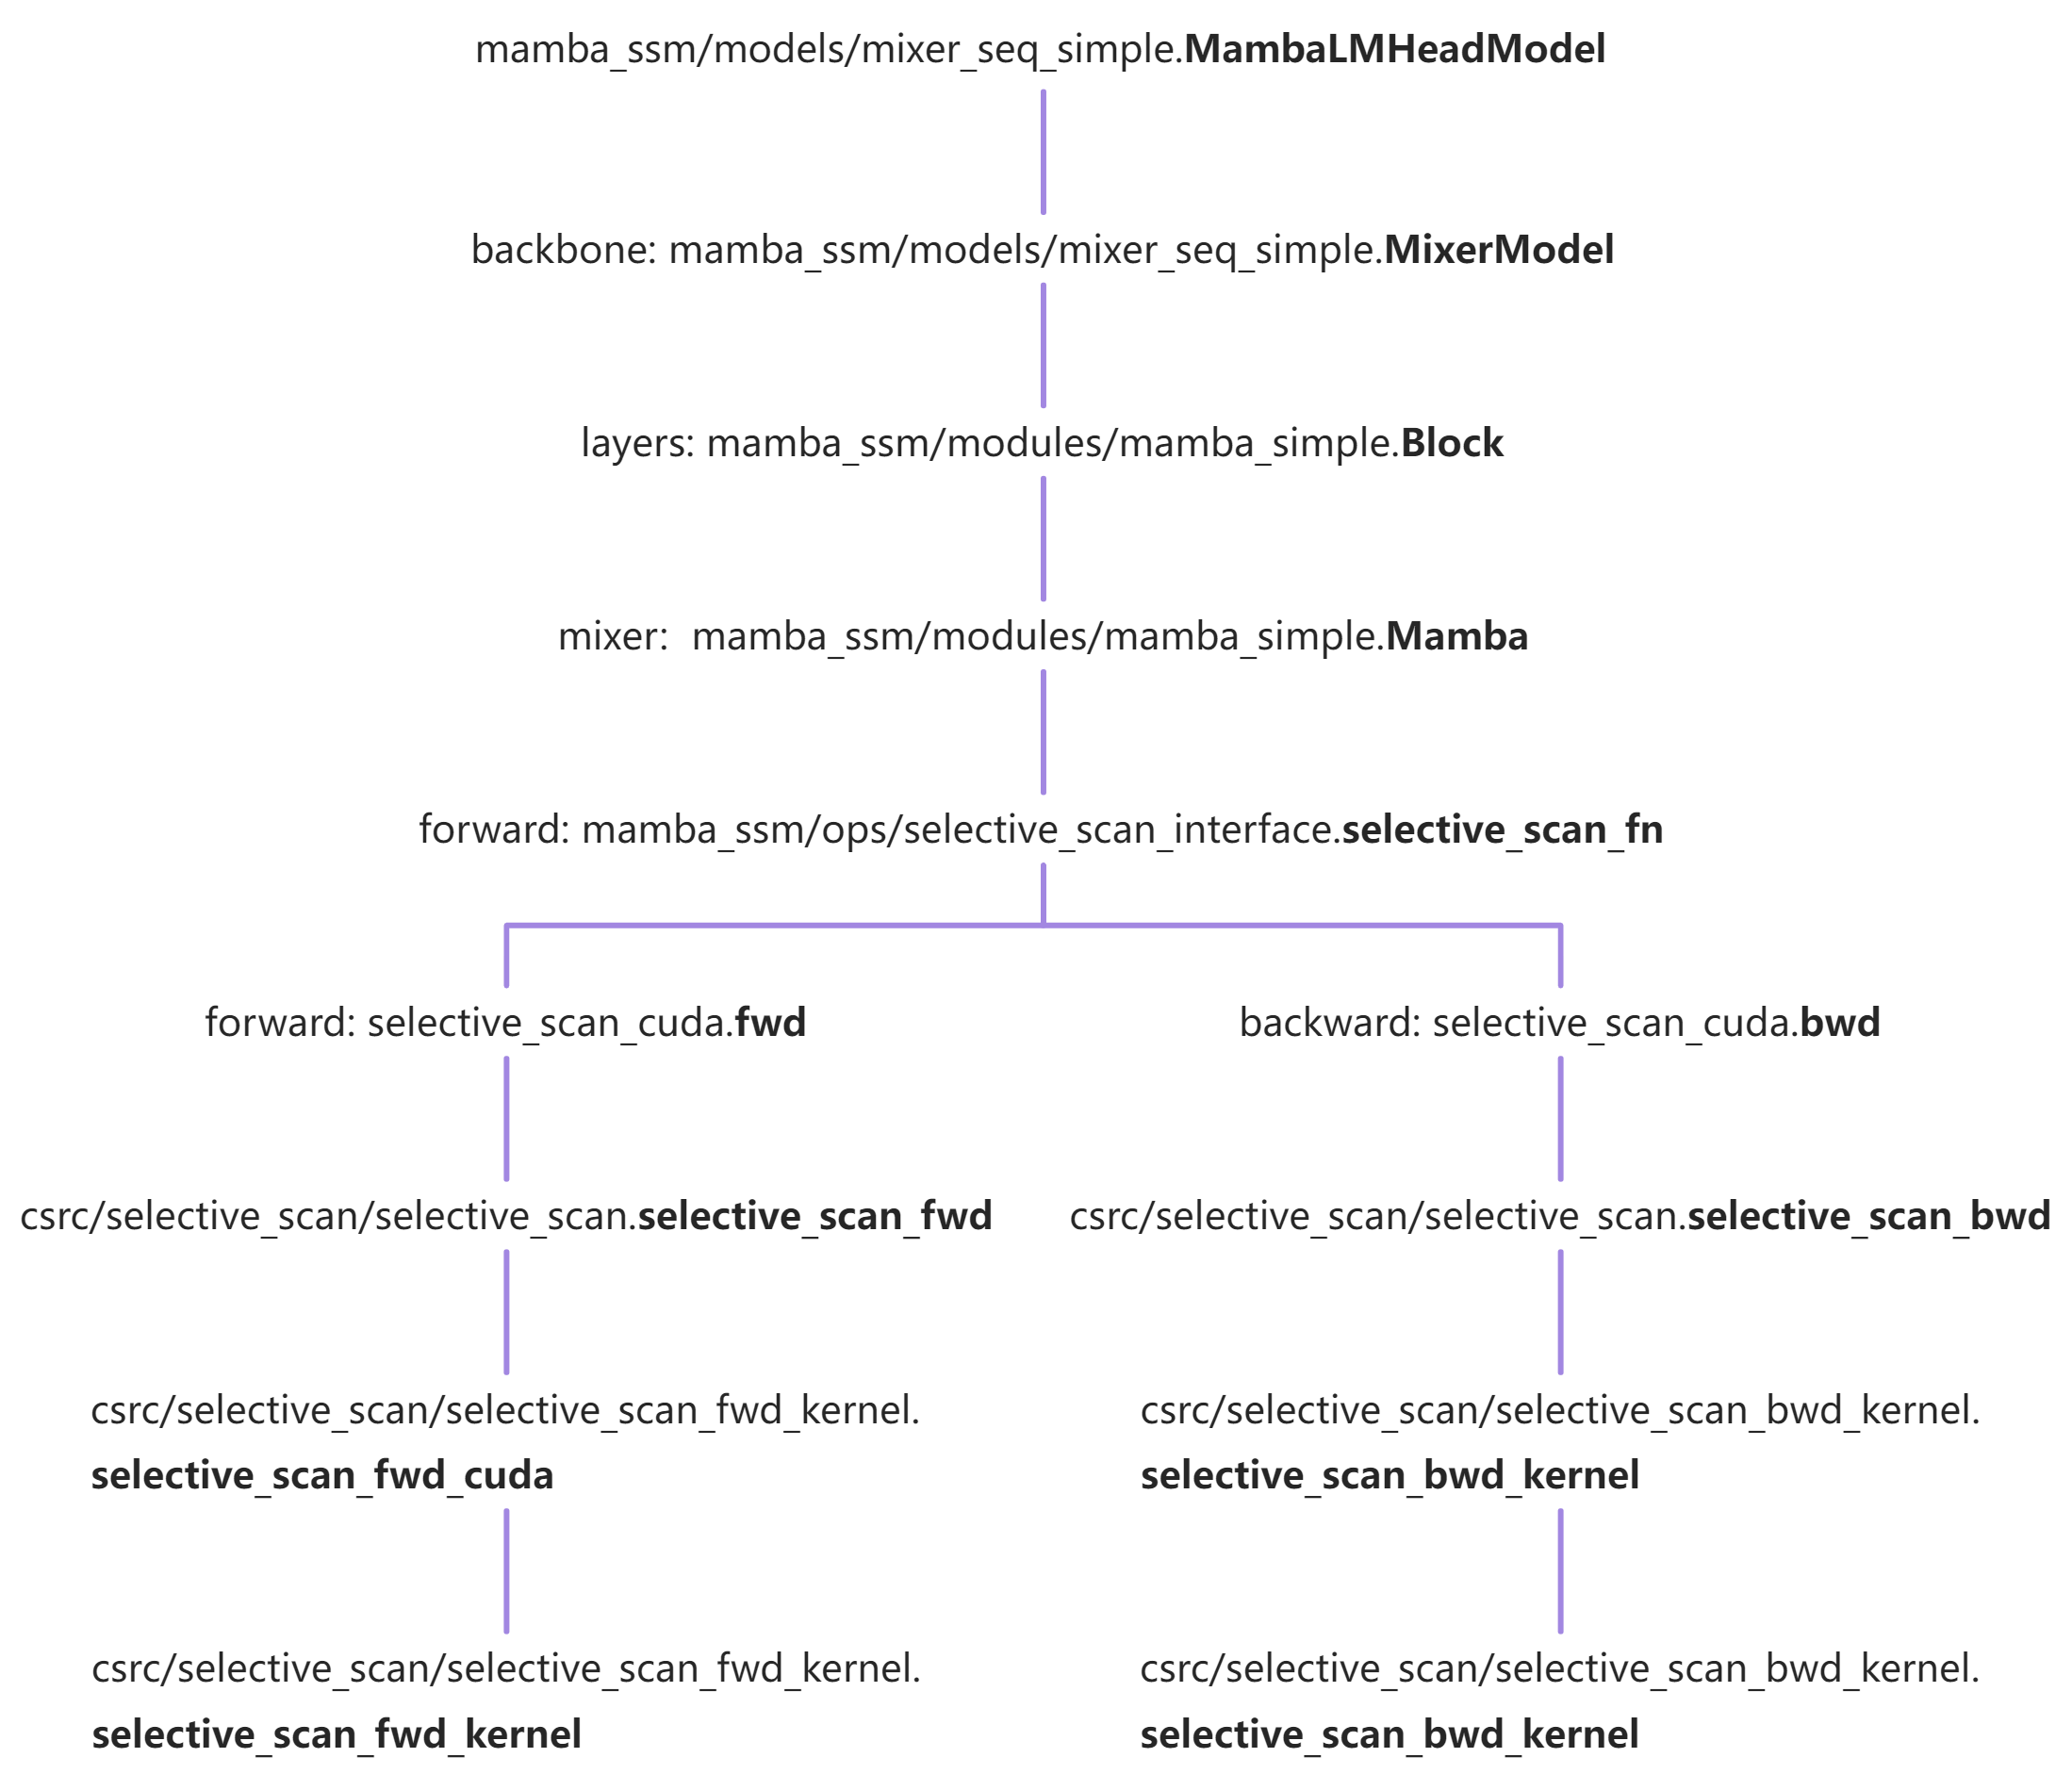
\includegraphics[width=0.95\textwidth]{figures/Mamba.png}
    \caption{Mamba代码结构}
    \label{fig:mamba_structure}
\end{figure}

% \begin{customquote}
%     这里是被引用的文章内容,显示为浅色字体。这可以是从其他文章中摘录的一段话,用于强调、讨论或解释。
% \end{customquote}

% \section{介绍}
% 这是一个支持中文的 LaTeX 模板,适用于展示代码和算法~\cite{knuth1984texbook}。

% \section{代码示例}
% 展示一个 Python 代码示例:

% \begin{lstlisting}[language=Python, caption=Python 示例代码]
% # Python 示例
% def hello_world():
%     print("Hello, world!")
% \end{lstlisting}

% 展示一个 CUDA C 代码示例:

% \begin{lstlisting}[style=cuda, caption=CUDA C 示例代码]
% // CUDA C 示例
% __global__ void hello_cuda() {
%     printf("Hello, CUDA!\n");
% }
% \end{lstlisting}

% \section{算法示例}
% 展示一个算法示例:

% \begin{algorithm}[H]
% \SetAlgoLined
% \KwResult{输出 "Hello, world!"}
%  初始化\;
%  \While{条件}{
%   "Hello, world!" 输出\;
%  }
%  \caption{算法示例}
% \end{algorithm}

\appendix
% \section{}
% 这里是附录A的内容,可以包含更多的代码示例、数据表格或额外的注释。

% 添加文献列表
\bibliographystyle{plain}
\bibliography{references}

\end{document}
